\subsection{Avvio Monitoraggio}\label{Avvio}

L'utente ha la possibilità di avviare il monitoraggio della rete bayesiana visualizzata al momento sul pannello \textit{G\&B} attraverso il pulsante \textbf{Avvio Monitoraggio} come si vede in Figura \ref{AvvioMonitoraggio}.

\begin{figure}[H]
	\begin{center}
		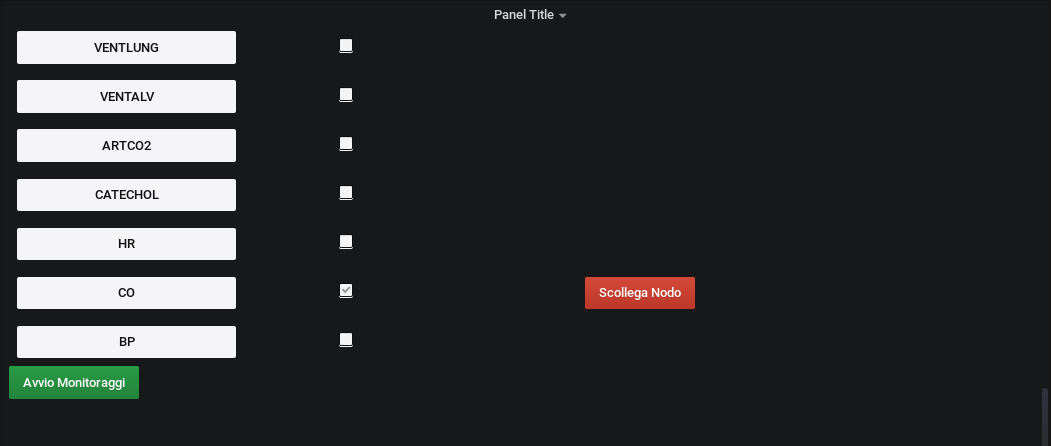
\includegraphics[scale=0.4]{./images/AvvioMonitoraggio.png}
		 \caption{Vista dell'Avvio del Monitoraggio}	
		 \label{AvvioMonitoraggio}
	\end{center}
\end{figure}

Affinchè il monitoraggio della rete possa essere avviato correttamente è necessario che l'utente abbia in precedenza completato tutte le necessarie operazioni di configurazione del collegamento della rete bayesiana al flusso di monitoraggio.\\
Nello specifico è necessario che l'utente, oltre ovviamente ad aver caricato una rete bayesiana (§\ref{ReteB}), deve aver:
\begin{itemize}
	\item Selezionato un database da usare come sorgente dei dati di monitoraggio (§\ref{SelectDB});
	\item Definito una politica temporale per il ricalcolo delle probabilità (§\ref{policy});
	\item Collegato almeno un nodo durante §\ref{Collegamento}.
\end{itemize} 

\pagebreak

\textbf{\textcolor{red}{ATTENZIONE}}: Nel caso in cui l'utente non abbia correttamente completato una delle operazioni precedentemente elencate il monitoraggio della rete non viene avviato e l'utente viene avvisato degli errori commessi da un messaggio di errore (Figura \ref{ErroreAvvio}).

\begin{figure}[H]
	\begin{center}
		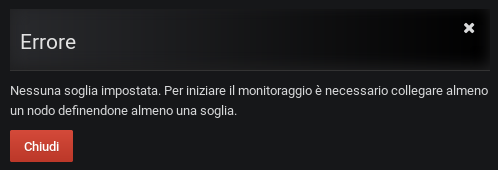
\includegraphics[scale=0.6]{./images/ErroreAvvio.png}
		 \caption{Messaggio di Errore Avvio Monitoraggio}	
		 \label{ErroreAvvio}
	\end{center}
\end{figure}

Nel caso in cui il cui, invece, l'avvio del monitoraggio dati sia andato a buon fine l'utente viene avvisato del buon esito dell'operazione attraverso un messaggio di notifica (Figura \ref{NotificaMonitoraggio}). La rete bayesiana, con le relative impostazioni di collegamento, viene inviata al server, il quale la memorizza e comincia ad eseguire le necessarie operazioni di ricalcolo delle probabilità per fornire all'utente dati di monitoraggio in tempo reale.

\begin{figure}[H]
	\begin{center}
		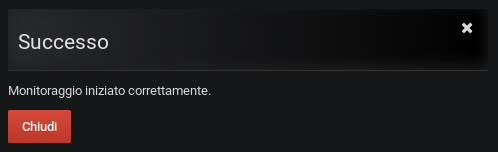
\includegraphics[scale=0.6]{./images/NotificaMonitoraggio.png}
		 \caption{Notifica di Avvio Monitoraggio Dati}	
		 \label{NotificaMonitoraggio}
	\end{center}
\end{figure}


